\documentclass[tikz, border=1pt]{standalone}
\usepackage{tikz}
\usetikzlibrary{arrows.meta, positioning}
\usepackage{xcolor,colortbl}
% Define extra colors
\definecolor{darkgreen}{rgb}{0.0, 0.5, 0.0} % Define a darker green

\begin{document}


\begin{figure}
    \centering

    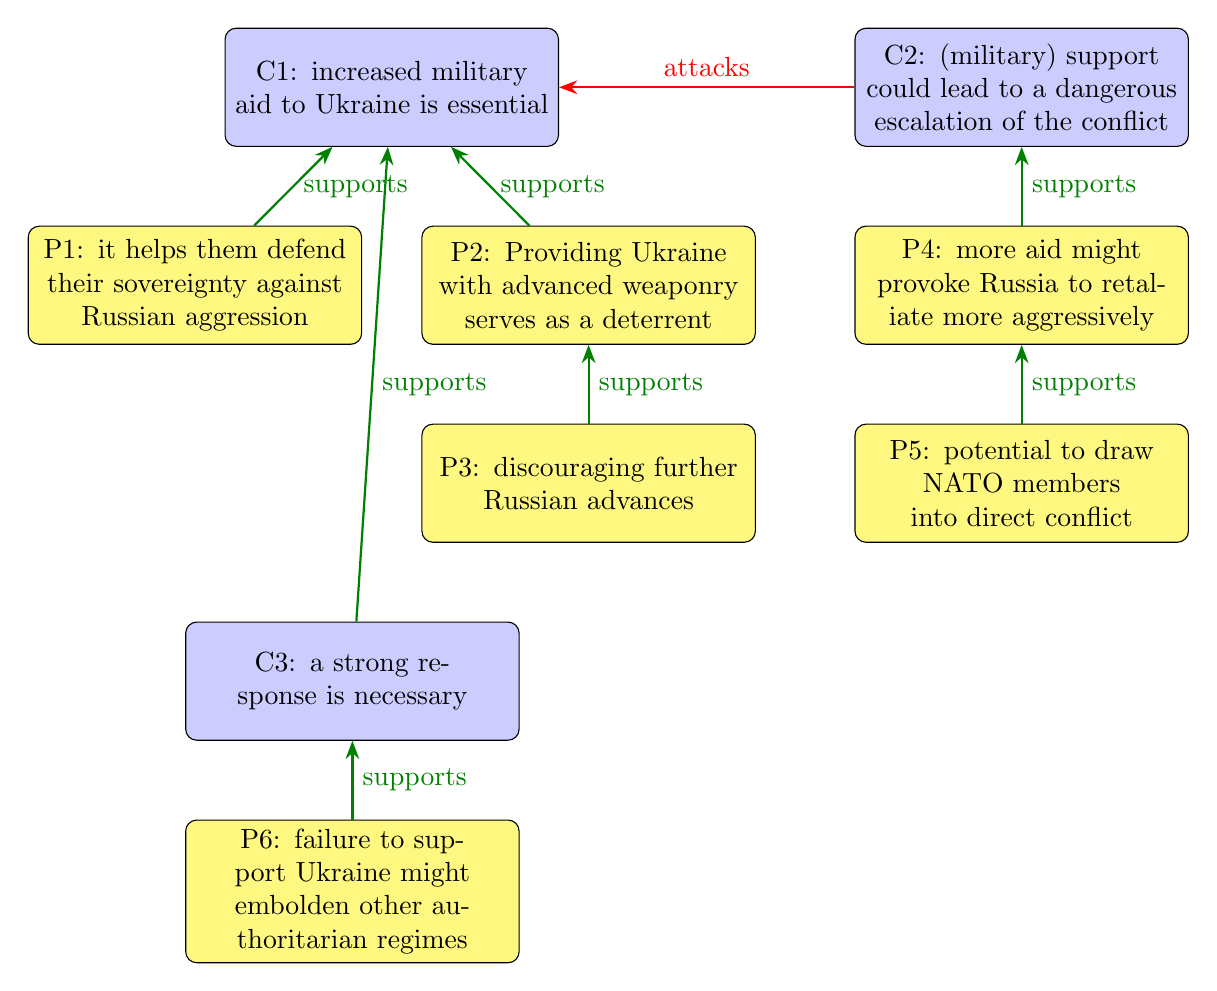
\begin{tikzpicture}[
        claim/.style={rectangle, draw, rounded corners, align=center, text width=4cm, minimum height=1.5cm, fill=blue!20},
        premise/.style={rectangle, draw, rounded corners, align=center, text width=4cm, minimum height=1.5cm, fill=yellow!50},
        arrow/.style={-{Stealth}, thick},
        support/.style={draw, -{Stealth}, thick, darkgreen},
        attack/.style={draw, -{Stealth}, thick, red},
        node distance=1cm and 1cm
        ]

        % Nodes
        \node (claim1) [claim, xshift=-4cm] {C1: increased military aid to Ukraine is essential};
        \node (premise1) [premise, below=of claim1, xshift=-2.5cm] {P1: it helps them defend their sovereignty against Russian aggression};
        \node (claim2) [claim, xshift=4cm] {C2: (military) support could lead to a dangerous escalation of the conflict};
        \node (premise2) [premise, below=of claim1, xshift=2.5cm] {P2: Providing Ukraine with advanced weaponry serves as a deterrent};
        \node (premise3) [premise, below=of premise2] {P3: discouraging further Russian advances};
        \node (premise4) [premise, below=of claim2] {P4: more aid might provoke Russia to retaliate more aggressively};
        \node (premise5) [premise, below=of premise4] {P5: potential to draw NATO members into direct conflict};
        \node (claim3) [claim, below=of premise3, xshift=-3cm] {C3: a strong response is necessary};
        \node (premise6) [premise, below=of claim3] {P6: failure to support Ukraine might embolden other authoritarian regimes};

        % Arrows with labels
        \draw [support] (premise1) -- node[midway, right] {supports} (claim1);
        \draw [attack] (claim2) -- node[midway, above] {attacks} (claim1);
        \draw [support] (premise2) -- node[midway, right] {supports} (claim1);
        \draw [support] (premise3) -- node[midway, right] {supports} (premise2);
        \draw [support] (claim3) -- node[midway, right] {supports} (claim1);
        \draw [support] (premise6) -- node[midway, right] {supports} (claim3);
        \draw [support] (premise4) -- node[midway, right] {supports} (claim2);
        \draw [support] (premise5) -- node[midway, right] {supports} (premise4);

    \end{tikzpicture}
\end{figure}

\end{document}